\chapter{Classificazione}\label{ch:classificazione}

\section{Introduzione}\label{sec:intro-class}
La \textbf{classificazione} suddivide un insieme di dati in \emph{classi} note a priori (etichette),
apprendendo da esempi etichettati come assegnare la classe a nuove tuple. È quindi
\emph{apprendimento supervisionato}. Al contrario, il \emph{clustering} non parte da etichette
(\emph{unsupervised}) e scopre gruppi per similarità.

\paragraph{Predizione (regressione).}
Quando il target è \emph{numerico continuo}, il compito è di \emph{predire} un valore reale
(apprendimento supervisionato \emph{continuo}), cercando una funzione che approssimi
il target, non un confine tra classi.

\subsection{Schema generale di un classificatore}\label{subsec:schema-class}
\begin{enumerate}
  \item \textbf{Costruzione del modello} (training): si apprende da un \emph{training set} etichettato.
  \item \textbf{Validazione/valutazione} (test): si misura la bontà su un \emph{test set} etichettato.
  \item \textbf{Uso} (deploy): si applica il modello a nuove tuple per predirne la classe.
\end{enumerate}

\paragraph{Overfitting.}
L’overfitting si verifica quando un modello “impara a memoria” il training, compreso il rumore: va molto bene sui dati visti ma generalizza male su dati nuovi. In pratica è un segnale che il modello è troppo complesso rispetto alle informazioni disponibili. Per ridurlo, si separano chiaramente i dati per la verifica e si preferiscono soluzioni più semplici quando offrono prestazioni simili.

\begin{figure}[htbp]
  \centering
  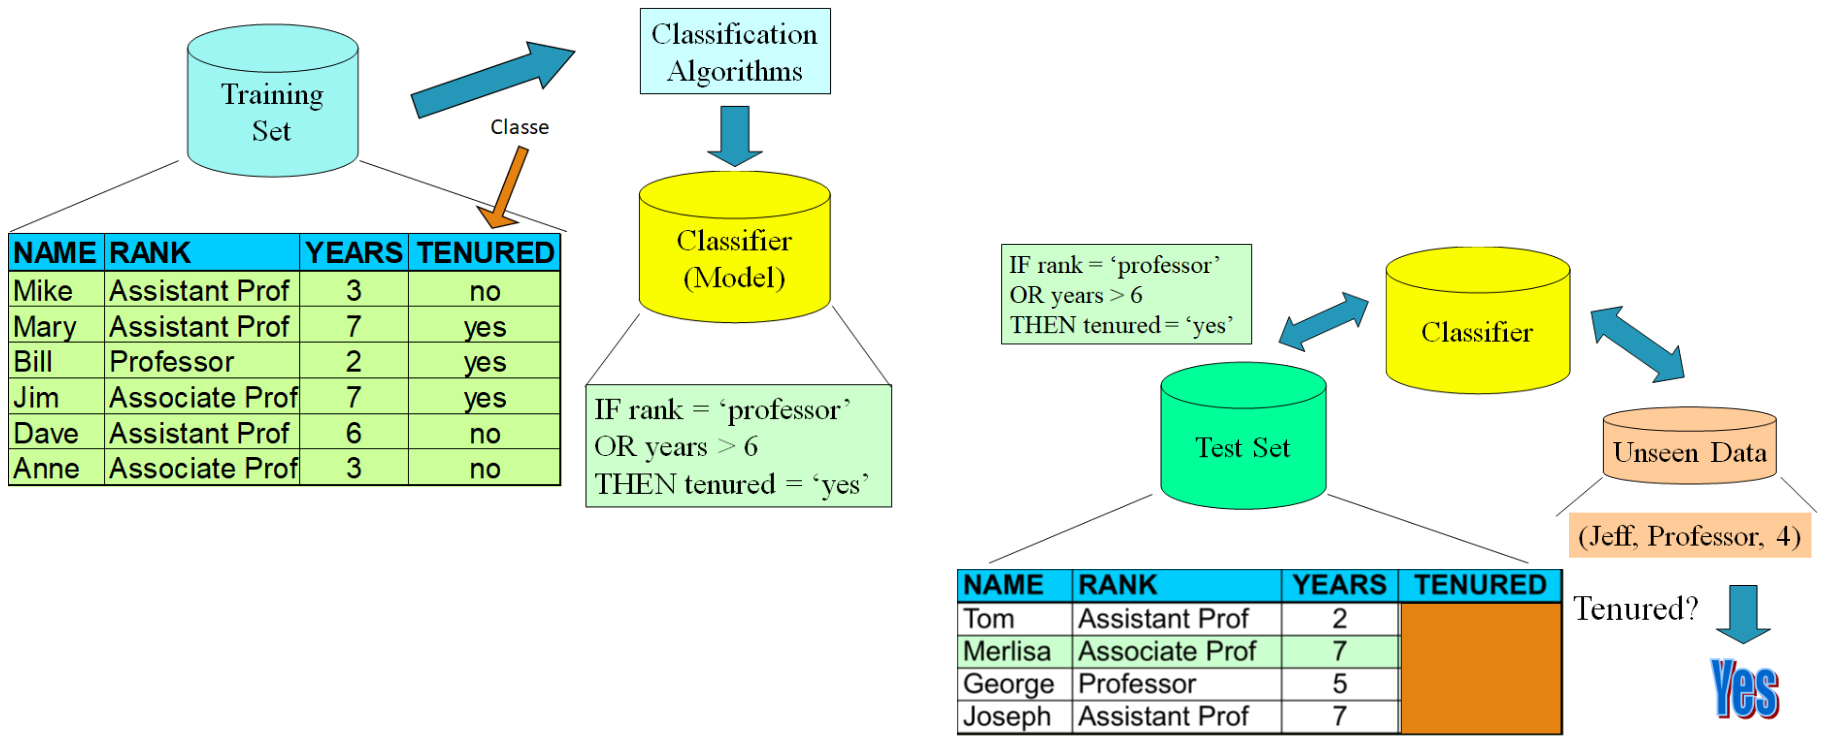
\includegraphics[width=.72\textwidth]{images/schema_classificatore.png}
  \caption{Schema a blocchi di un classificatore: addestramento, validazione e uso.}
  \label{fig:schema-class}
\end{figure}

\subsection{Requisiti desiderabili}\label{subsec:req}
\begin{itemize}
  \item \textbf{Accuratezza}: corretta predizione delle classi (o del valore, per i predittori).
  \item \textbf{Velocità}: tempi di training e di classificazione contenuti.
  \item \textbf{Robustezza}: tolleranza a rumore e dati mancanti.
  \item \textbf{Scalabilità}: efficienza su dataset di grandi dimensioni.
\end{itemize}

% ==========================================================
\section{Alberi decisionali}\label{sec:trees}
Gli \textbf{alberi decisionali} classificano applicando test su attributi lungo i nodi interni;
le \emph{foglie} portano le etichette di classe.

\subsection{Classificazione tramite albero}\label{subsec:tree-class}
La classe di una tupla $q$ si ottiene seguendo il cammino radice$\to$foglia guidato
dai test. Ogni cammino implementa una regola \texttt{IF-THEN} (le condizioni interne sono congiunte in AND). L’insieme di regole è \emph{esaustivo} e \emph{mutuamente esclusivo} (ogni tupla è coperta da una sola regola).

\begin{figure}[htbp]
  \centering
  \begin{minipage}[t]{.50\textwidth}
    \centering
    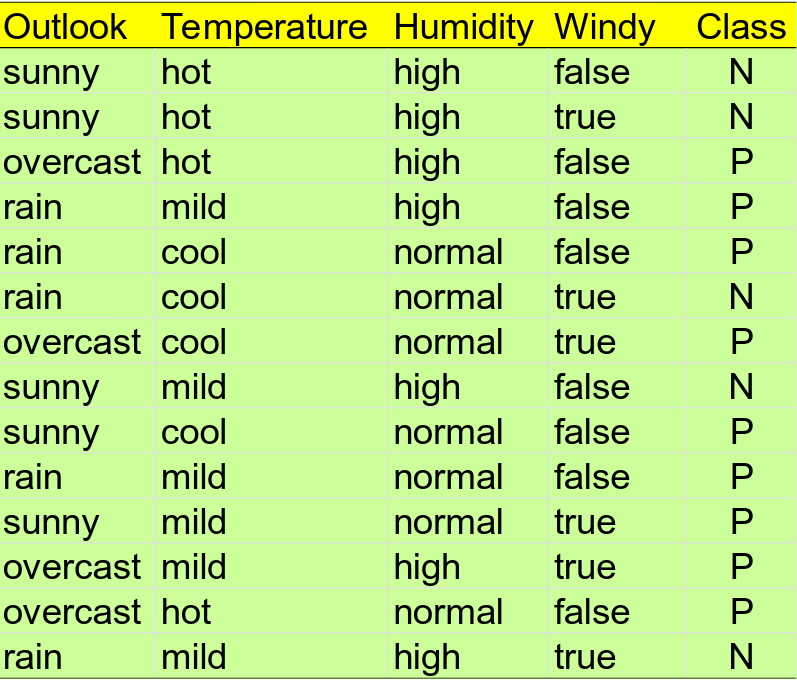
\includegraphics[width=\linewidth]{images/weather_table.png}
  \end{minipage}\hfill
  \begin{minipage}[t]{.48\textwidth}
    \centering
    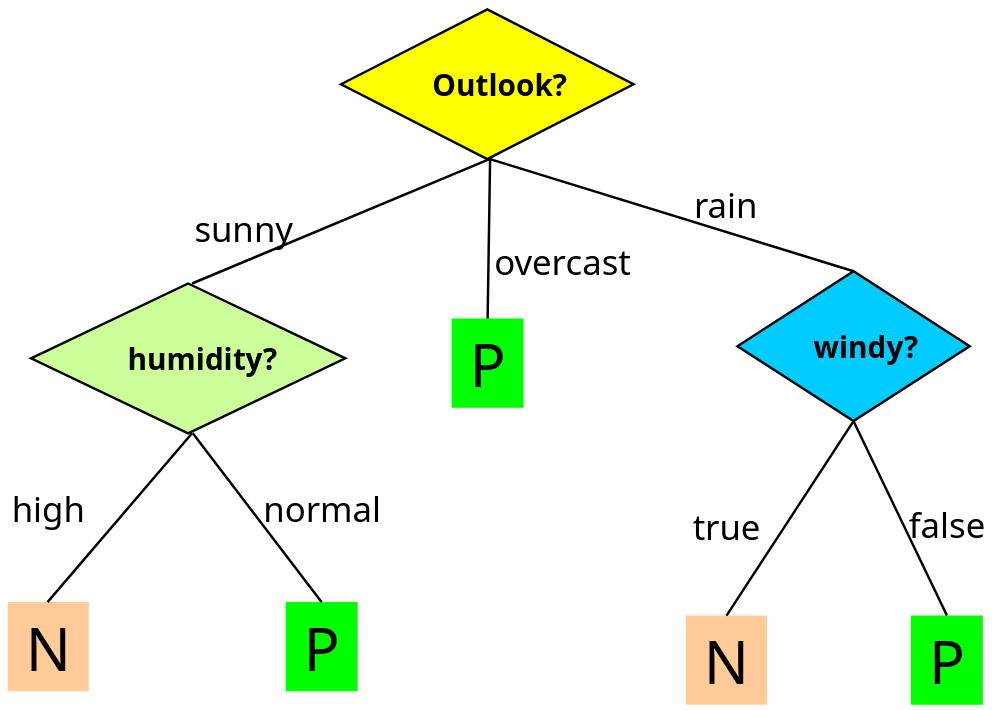
\includegraphics[width=\linewidth]{images/decision_tree_weather.png}
  \end{minipage}
  \caption{Dataset \emph{weather} (a sinistra) e albero decisionale appreso (a destra). 
  La tabella contiene 14 esempi con quattro attributi descrittivi (\texttt{Outlook}, \texttt{Temperature}, 
  \texttt{Humidity}, \texttt{Windy}) e la classe binaria \texttt{P/N}. 
  L’albero (stile ID3/C4.5) sceglie come radice \texttt{Outlook}; il ramo \texttt{overcast} porta 
  direttamente alla classe \texttt{P}, mentre per \texttt{sunny} si testa \texttt{Humidity} e per \texttt{rain} 
  si testa \texttt{Windy}. L’esempio illustra il passaggio da dati tabellari a regole interpretabili.}
  \label{fig:weather-tree}
\end{figure}

\subsection{Costruzione top–down}\label{subsec:topdown}
Costruzione ricorsiva dalla radice:
\begin{enumerate}
  \item Se tutte le tuple del nodo $X$ hanno la \emph{stessa} classe $C$, crea una foglia $C$.
  \item Altrimenti scegli un attributo $A$ (non ancora usato) e \emph{ramifica} $X$ (\emph{splitting}) secondo i valori/soglia di $A$; crea i figli.
  \item Per ogni figlio $X_i$: se puro, fermati; se impuro, ripeti ricorsivamente.
\end{enumerate}

\paragraph{Pruning.}
Se le tuple nel nodo sono poche o la profondità è elevata, si può fermare prima e rendere il nodo una foglia (vedere figura \ref{fig:weather-tree} con l'attributo "overcast").

\subsection{Splitting degli attributi}\label{subsec:splitting}
\begin{itemize}
  \item \textbf{Booleani/numerici}: split \emph{binario} su soglia $t$ (``$\le t$'' a sinistra, ``$>t$'' a destra).
  \item \textbf{Categoriali}: split \emph{binario} definendo un sottoinsieme non vuoto di valori (a sinistra se il valore \emph{non} appartiene al sottoinsieme, a destra altrimenti).
\end{itemize}

\subsection{Scelta dell’attributo e strategia greedy}\label{subsec:greedy}
L’albero minimale è un problema \emph{NP-hard}; si usa una strategia \emph{greedy} che, ad ogni passo, seleziona l’attributo con massima \emph{goodness} (partizioni più pure),
costruendo l’albero “più compatto” possibile.

\section{Misure di goodness}\label{sec:goodness}
La scelta dell’attributo si basa su misure di \emph{goodness}, che variano da algoritmo ad algoritmo.

\subsection{Information Gain (ID3)}\label{subsec:ig}
\paragraph{Idea.} L'\textbf{Information gain} è un algoritmo che si basa sull'idea di selezionare l'attributo che massimizza la riduzione dell'entropia riguardo alla classe delle tuple dopo lo split. Questo perché:
\begin{itemize}
  \item \textbf{Entropia massima}: si ha quando le classi sono equamente distribuite (massima incertezza).
  \item \textbf{Entropia minima}: si ha quando tutte le tuple appartengono alla stessa classe (certezza completa). 
\end{itemize}

\noindent
Sia $S_X$ l’insieme di tuple al nodo $X$, con due classi $P$ e $N$; si indichino con $p$
e $n$ le rispettive numerosità. L’\textbf{entropia} di $S_X$ è
\[
H(S_X)\;=\; -\frac{p}{p+n}\log_2\!\frac{p}{p+n}\;-\;\frac{n}{p+n}\log_2\!\frac{n}{p+n}.
\]
Sia $A$ un attributo con $k$ valori distinti, che induce la partizione
$S_X \to S_1,\dots,S_k$. Se $S_i$ contiene $p_i$ e $n_i$ elementi, allora
\[
H(S_i)\;=\; -\frac{p_i}{|S_i|}\log_2\!\frac{p_i}{|S_i|}\;-\;\frac{n_i}{|S_i|}\log_2\!\frac{n_i}{|S_i|}
\]

Possiamo anche calcolare l'\textbf{entropia media} dopo lo split su $A$:
\[
\overline{H}_A(S_X)\;=\;\sum_{i=1}^k \frac{|S_i|}{|S_X|}\,H(S_i).
\]

L’\textbf{information gain} è definito come la riduzione di entropia ottenuta dal partizionamento $S_x$ scegliendo l'attributo $A$:
\[
\mathrm{Gain}(S_X,A)\;=\;H(S_X)\;-\;\overline{H}_A(S_X).
\]
Si sceglie l’attributo con gain massimo.

\subsubsection*{Esempio e limitazioni}\label{par:ig-example}
Sul dataset “weather” (Fig.~\ref{fig:weather-tree}) si ottengono:
\[
\mathrm{Gain}(\textit{outlook})=0.246,\quad
\mathrm{Gain}(\textit{temperature})=0.029,\quad
\mathrm{Gain}(\textit{humidity})=0.151,\quad
\mathrm{Gain}(\textit{windy})=0.048.
\]

\paragraph{Limite noto.} L’Information Gain è \emph{sbilanciato} verso attributi con molti valori:
un attributo quasi univoco (es.\ \texttt{ID}) produce molte partizioni piccole (foglie pure),
abbattendo l’entropia media e gonfiando artificialmente , pur senza reale capacità
predittiva.

\begin{figure}[htbp]
  \centering
  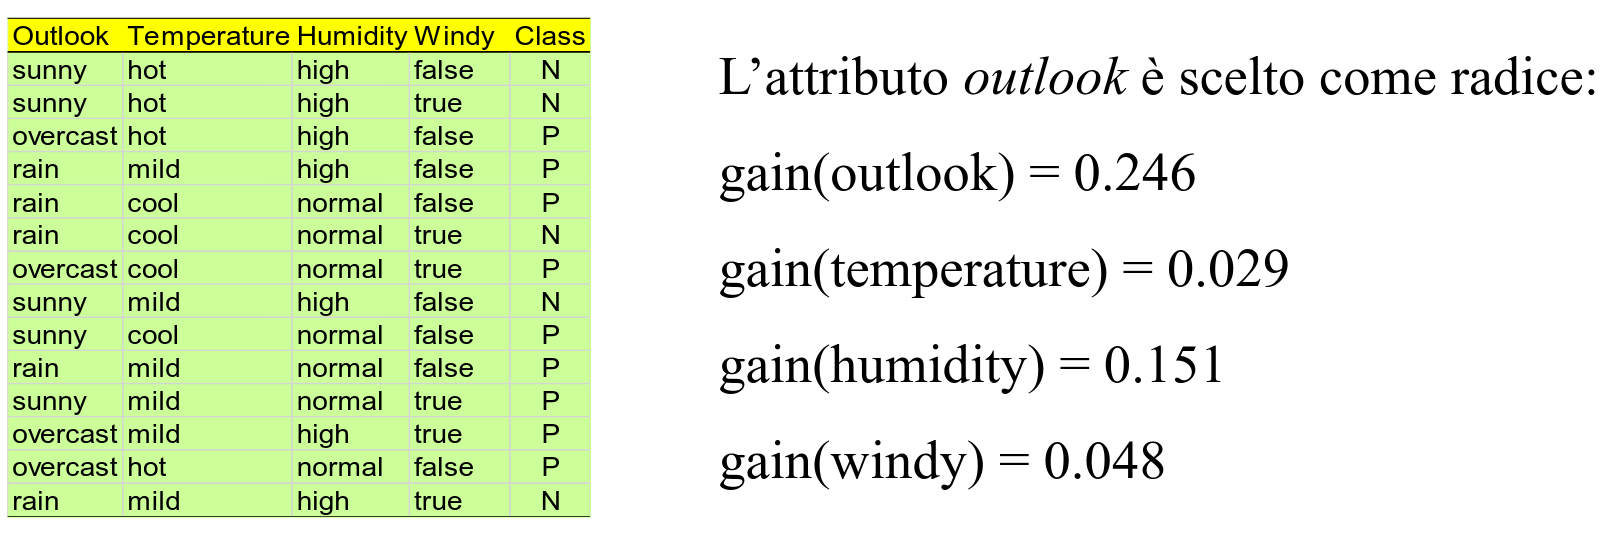
\includegraphics[width=.9\textwidth]{images/ig_outlook_example.png}
  \caption{Esempio di scelta della radice con Information Gain sul dataset “weather”.}
  \label{fig:ig-weather}
\end{figure}

\subsection{Gain Ratio (C4.5)}\label{subsec:gain-ratio}
Il \textbf{Gain Ratio} corregge il bias dell’Information Gain verso attributi con molti valori introducendo la \emph{split information}, che misura quanta informazione è generata dal solo atto di partizionare i dati secondo l’attributo (indipendentemente dalla classe).

Sia $S$ l’insieme di tuple nel nodo corrente e $A$ un attributo che induce la partizione $S=S_1\cup\cdots\cup S_k$. Definiamo
\[
\mathrm{SplitInfo}(A,S)
= -\sum_{i=1}^k \frac{|S_i|}{|S|}\,\log_2\!\Big(\frac{|S_i|}{|S|}\Big),
\qquad
\mathrm{Gain}(A,S)=H(S)-\sum_{i=1}^{k}\frac{|S_i|}{|S|}\,H(S_i).
\]
Il \textbf{Gain Ratio} è
\[
\mathrm{GR}(A,S)=\frac{\mathrm{Gain}(A,S)}{\mathrm{SplitInfo}(A,S)}.
\]
\paragraph{Selezione in C4.5.} Per evitare divisioni spurie quando $\mathrm{SplitInfo}$ è piccola, C4.5 sceglie l’attributo con $\mathrm{GR}$ massimo tra quelli con \emph{Gain} non inferiore (ad es.) al gain medio del nodo. In pratica:
\begin{enumerate}
  \item calcola $\mathrm{Gain}(A,S)$ e scarta attributi con gain $\le 0$;
  \item tra i rimanenti, seleziona l’attributo con $\mathrm{GR}$ più alto.
\end{enumerate} 

\paragraph{Nota pratica (attributi continui).}
Per un attributo numerico $A$ si ordinano i valori e si valutano soglie candidate $t$ nelle posizioni fra due valori consecutivi: $A\le t$ vs $A>t$. Per ogni soglia si calcolano gain e gain ratio; si sceglie la soglia che massimizza la metrica.

% --------------------------------------------------------------------

\subsection{Gini Index (CART)}\label{subsec:gini}
Sia $i$ una classe e $T$ una tupla di classe $i$ scelta a caso da $S_x$. Per ricavare il \textbf{Gini Index} si calcola la probabilità che $T$ venga classificata erroneamente, ovvero che appartenga a una classe diversa da $i$: e quindi occorre considerare:
\begin{itemize}
  \item \textbf{Probabilità che $T$ sia di classe $i$}: $P(i\mid S_X)$.
  \item \textbf{Probabilità che $T$ sia di una classe diversa da $i$}: $1 - P(i\mid S_X)$.
\end{itemize}

\noindent
Dato che il ragionamento fatto vale per ogni classe, si sommano le probabilità di errore su tutte le classi:  
\[
\mathrm{Gini}(S_X) = \sum_{i=1}^n p_i (1-p_i) = \sum_{i=1}^n (p_i-p_i^2) = \sum_{i=1}^n p_i - \sum_{i=1}^n p_i^2 = 1 - \sum_{i=1}^n p_i^2 
\]

Con la supposizione che $S_x$ contenga $k$ classi e che $p_i$ sia la probabilità che una tupla scelta a caso da $S_X$ appartenga alla classe $i$, si ha che il \textbf{Gini Index} dello split è defininito come:
\[
\mathrm{Gini_{split}}(S_X) = 1 - \sum_{i=1}^k \frac{|S_i|}{|S_x|}Gini(S_i) 
\]

CART seleziona l’attributo/soglia che \emph{minimizza} $\mathrm{GiniSplit}$. Su attributi categoriali si cercano partizioni in due sottoinsiemi di valori; su continui, soglie come in C4.5.

% --------------------------------------------------------------------

\subsection{Pruning degli alberi}\label{subsec:pruning}
Alberi molto profondi generalizzano male (generano \emph{overfitting}). Per evitare questo, si effettua un \textbf{pruning}, ovvero si riduce la dimensione dell'albero sostituendo un sottoalbero con una foglia etichettato con la classe maggioritaria delle tuple nel sottoalbero, il pruning inserisce però un tasso di errore, si fa solo se necessario. Si usano due strategie principali:
\begin{description}
  \item[Pre-pruning] in fase di costruzione dell'albero si interrompe la crescita quando la goodness dello split è al di sopra di una \emph{soglia}.
  \item[Post-pruning] si costruisce l'albero completo e poi lo si riduce valutando l'errore su validation set o tramite stima incrociata. Generalmente è più dispensioso ma più efficace.
\end{description}

\subsubsection*{Pruning pessimistico (C4.5)}
Confronta l’errore stimato del \emph{sottoalbero} $T$ radicato in $X$ con l’errore stimato della \emph{foglia} che sostituisce $T$ (classe maggioritaria in $X$).

Sia \(X\) un nodo dell’albero con insieme di esempi \(S_x\) (\(N=|S_x|\)) e classe di maggioranza \(C\).
Sia \(T\) il sottoalbero radicato in \(X\) e siano \(x_1,\dots,x_k\) i figli immediati di \(X\), con
\(S_{x_i}\) gli esempi nel figlio \(x_i\) e \(C_i\) la sua classe di maggioranza. Le due quantità
\[
\begin{aligned}
E_p(T)   &= \frac{\bigl|\{\, t \in S_x \mid \mathrm{class}(t) \neq C \,\}\bigr| + \epsilon}{\lvert S_x\rvert}\\[4pt]
E_p'(T) &= \frac{\displaystyle \sum_{i=1}^{k} \bigl|\{\, t \in S_{x_i} \mid \mathrm{class}(t) \neq C_i \,\}\bigr| + k\,\epsilon}{\lvert S_x\rvert}
\end{aligned}
\]
sono le \textbf{stime del tasso di errore} usate per decidere se fare pruning.

\paragraph{Che cosa misurano.}
\begin{itemize}
  \item \(E_p(T)\) è l’\emph{errore stimato} se \textbf{si pota} \(T\) sostituendo l’intero sottoalbero con \emph{una sola foglia} etichettata con la classe di maggioranza \(C\) del nodo \(X\). Il numeratore conta le istanze di \(S_x\) che verrebbero sbagliate da tale foglia, con una \emph{correzione} \(\epsilon\) (tipicamente \(\epsilon=\tfrac12\)) per evitare stime troppo ottimistiche su campioni piccoli.
  \item \(E_p'(T)\) è l’\emph{errore stimato} se \textbf{si mantiene lo split corrente} di \(X\) nei suoi \(k\) figli, ma \emph{troncando} ognuno di essi a foglia (ognuna etichettata con la propria maggioranza \(C_i\)). Si sommano gli errori dei \(k\) figli e si aggiunge una correzione \(\epsilon\) per \emph{ciascuna} foglia (\(k\epsilon\)).
\end{itemize}

\paragraph{Decisione di pruning.}
Confrontando \(E_p(T)\) ed \(E_p'(T)\):
\begin{itemize}
  \item per \(E_p(T) \le E_p'(T)\), \emph{potare} il nodo \(X\) è preferibile, poiché l’errore stimato come foglia è minore o uguale a quello del sottoalbero.
  \item per \(E_p(T) > E_p'(T)\), conviene \emph{mantenere} lo split, in quanto l’errore stimato del sottoalbero è inferiore a quello della singola foglia.
\end{itemize}

Il valore $\epsilon$ è una sorta di “costo fisso” per ogni foglia aggiunta all’albero. L’aggiunta di questo valore agisce da \emph{regolarizzatore}: penalizza strutture con molte foglie, evitando che piccole fluttuazioni del campione giustifichino split inutili.

\subsubsection*{Cost–complexity pruning (CART)}
Si valuta il vantaggio dello \emph{split} di un nodo \(X\) confrontando la riduzione di \emph{error rate} con l’aumento di complessità (nuove foglie).

\paragraph{Errore prima e dopo lo split.}
Sia \(S_X\) l’insieme dei campioni che arrivano al nodo \(X\) e \(C\) la classe maggioritaria in \(S_X\).
\[
E(X)=\frac{\bigl|\{\,t\in S_X:\ \mathrm{class}(t)\neq C\,\}\bigr|}{|S_X|}.
\]
Se \(X\) viene diviso in \(k\) figli \(X_1,\dots,X_k\) (con classi maggioritarie \(C_1,\dots,C_k\)), l’errore \emph{atteso dopo} lo split è
\[
E'(X)=\frac{\sum_{i=1}^{k}\bigl|\{\,t\in S_{X_i}:\ \mathrm{class}(t)\neq C_i\,\}\bigr|}{|S_X|}.
\]

\paragraph{Indice di costo–complessità per lo split.}
Definiamo il guadagno medio per foglia aggiunta:
\[
\alpha(X)=\frac{E(X)-E'(X)}{k-1}.
\]

Il valore \(\alpha\) misura \emph{quanto} diminuisce l’errore per ogni foglia extra introdotta dallo split. Se \(\alpha\) è sufficientemente piccolo, ovvero quando $\alpha$ è minore di una soglia prefissata \(\alpha_0\), lo split non è conveniente e si pota il nodo \(X\).

\begin{figure}[htbp]
  \centering
  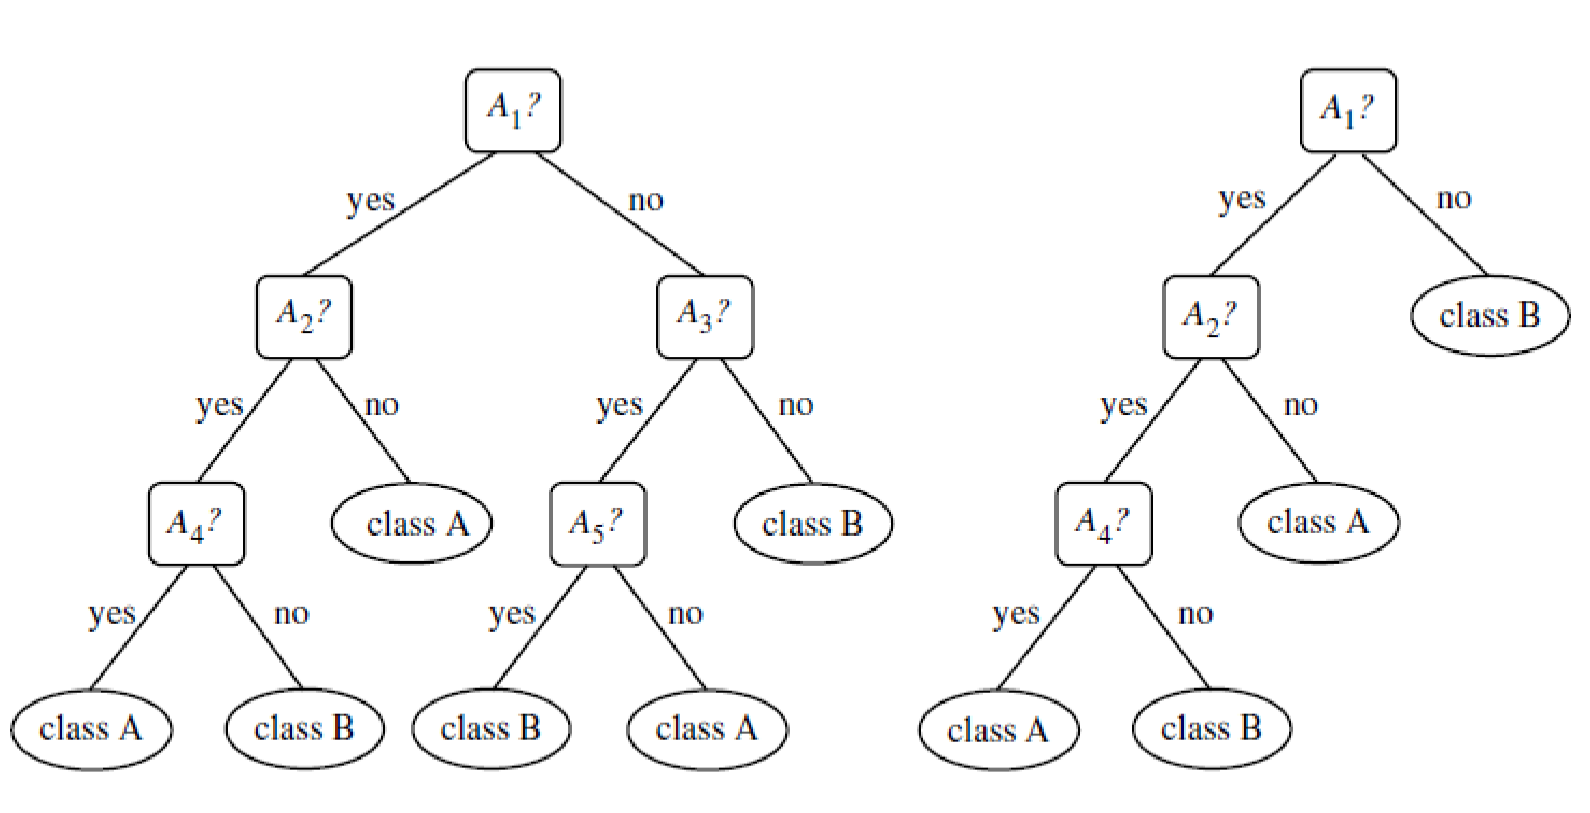
\includegraphics[width=.75\textwidth]{images/tree_pruning_example.png}
  \caption{Pruning: confronto errore stimato del sottoalbero vs foglia (C4.5) e principio costo–complessità (CART).}
  \label{fig:pruning}
\end{figure}

\paragraph{Pro/contro degli alberi decisionali.}
\emph{Pro:} interpretabili, veloci in predizione, gestiscono mix di attributi (continui/categoriali), poca preparazione dei dati. \emph{Contro:} instabili rispetto a piccole variazioni dei dati, propensi all’overfitting, separazioni per soglie assiali (forme complesse richiedono molti nodi), accuratezza spesso inferiore a ensemble o SVM su dati ad alta dimensionalità.

% --------------------------------------------------------------------

\section{Classificatori generativi}\label{sec:generative}
I modelli generativi producono un \textbf{modello probabilistico} a partire dai dati, predicendo la \textbf{classe} di appartenenza \emph{più probabile} per un nuovo dato a partire dal modello sviluppato. Questi modelli si basano sul \textbf{teorema di Bayes}.

\subsection{Teorema di Bayes e regola di decisione}\label{subsec:bayes-rule}
Sia $\mathbf{x}$ un’osservazione e $c\in\mathcal{C}$ una classe candidata. Per decidere la
classe usiamo il \textbf{teorema di Bayes}:
\[
P(c\mid \mathbf{x})=\frac{P(\mathbf{x}\mid c)\,P(c)}{P(\mathbf{x})}.
\]
\begin{itemize}
  \item \textbf{Probabilità a priori} $P(c)$: quanto la classe $c$ è probabile \emph{prima} di vedere i dati (in pratica: frequenza della classe nel train).
  \item \textbf{Likelihood} $P(\mathbf{x}\mid c)$: quanto è plausibile osservare $\mathbf{x}$ \emph{se} la classe fosse $c$.
  \item \textbf{Evidenza} $P(\mathbf{x})$: probabilità complessiva di osservare $\mathbf{x}$ (uguale per tutte le classi).
\end{itemize}
La decisione ottima \emph{MAP} (Maximum A Posteriori) è
\[
\hat{c}(\mathbf{x})=\arg\max_{c\in\mathcal{C}} P(c\mid \mathbf{x})
=\arg\max_{c\in\mathcal{C}} P(\mathbf{x}\mid c)\,P(c),
\]
poiché $P(\mathbf{x})$ non dipende da $c$ e non influisce sull’$\arg\max$.
\subsection{Naive Bayes}\label{subsec:naive-bayes}
\paragraph{Idea.}
Assumiamo che, fissata la classe \(c\), le feature siano indipendenti (\emph{assunzione naive}). Allora la verosimiglianza fattorizza:
\[
P(\mathbf{x}\mid c)=\prod_{j=1}^{d} P(x_j\mid c).
\]

\paragraph{Regola di decisione (MAP, in scala logaritmica).} Le probabilità condizionali sono molto piccole e un prodotto di tante quantità prossime a 0 può portare problemi di underflow. Per ovviare a questi problemi si considera il \textbf{log-likelihood}:
\[
\hat{c}(\mathbf{x})=\arg\max_{c\in\mathcal{C}}
\Big[\log P(c)+\sum_{j=1}^{d}\log P(x_j\mid c)\Big].
\]

\noindent
Questo si traduce in una somma anziché in un prodotto di termini.

\paragraph{Stima essenziale delle probabilità.}
\begin{itemize}
  \item \textbf{Prior} \(P(c)\): frequenza della classe nel training.
  \item \textbf{Attributi discreti}: frequenze condizionate con \emph{Laplace smoothing} \((+\alpha)\) per evitare zeri.
  \item \textbf{Attributi continui}: modello gaussiano per \(x_j\mid c\) con media e varianza stimate sui dati della classe.
\end{itemize}

\paragraph{Vantaggi e svantaggi.} Molto veloce e facile da implementare, l'assunzione di indipendenza condizionale potrebbe non essere sempre vera e potrebbe portare ad una perdita di accuratezza (tali dipendenze non possono essere modellate da questo modello).
% --------------------------------------------------------------------

\subsection{Reti Bayesiane}\label{subsec:bayesnet}
Una \textbf{rete bayesiana} è un DAG le cui variabili $\{X_1,\dots,X_d\}$ fattorizzano come
\[
P(X_1,\dots,X_d)=\prod_{i=1}^d P(X_i\mid \mathrm{Pa}(X_i)),
\]
dove $\mathrm{Pa}(X_i)$ sono i genitori di $X_i$ nel grafo. Il DAG codifica indipendenze condizionali; i CPT (tabelle di probabilità condizionate) specificano i parametri.

\begin{figure}[htbp]
  \centering
  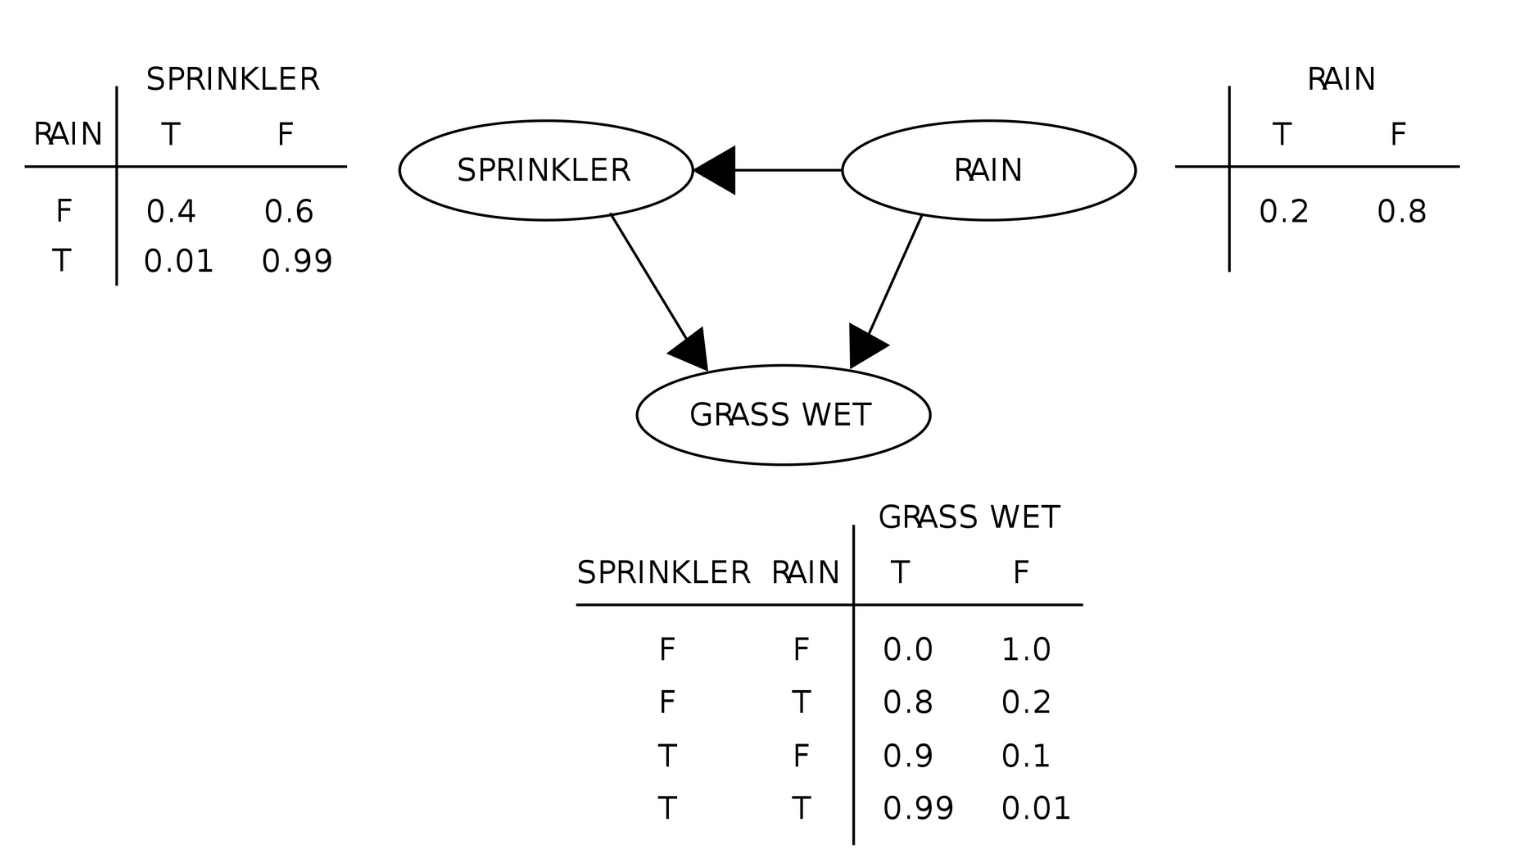
\includegraphics[width=.9\textwidth]{images/bayes_network_example.png}
  \caption[Bayes net Sprinkler–Rain–Grass]{Rete bayesiana \emph{Sprinkler–Rain–Grass}: il DAG orientato specifica le dipendenze e indetermina la fattorizzazione della congiunta
  \(P(\text{Rain})\,P(\text{Sprinkler}\mid \text{Rain})\,P(\text{GrassWet}\mid \text{Sprinkler},\text{Rain})\).
  Le tabelle mostrano le CPD (Conditional Probability Tables) dei nodi.
  A differenza di Naive Bayes, le feature possono essere dipendenti dato la/e causa/e (qui \textit{Rain}), e tale dipendenza è resa esplicita dagli archi.}
  \label{fig:bayes-net}
\end{figure}

\paragraph{Uso per la classificazione.}
Dato $\mathbf{x}$, si calcolano (o si approssimano) $P(y\mid \mathbf{x})$ tramite inferenza sul DAG (\emph{esatta} o \emph{approx} con sampling/variational). Le reti bayesiane generalizzano Naive Bayes (che è un caso particolare con $Y$ genitore di tutte le feature e nessun’altra dipendenza).

\section{Classificatori discriminativi}\label{sec:discriminativi}
I classificatori discriminativi stimano direttamente una funzione di decisione $f:\mathbb{R}^d\to\mathbb{R}$ (o, opzionalmente, la probabilità condizionata $P(y\mid\mathbf{x})$) senza modellare la distribuzione congiunta $P(\mathbf{x},y)$. Dato un nuovo esempio $\mathbf{x}$ si valuta $f(\mathbf{x})$ e si assegna l'etichetta corrispondente. Rispetto ai modelli generativi richiedono generalmente meno assunzioni sui dati. Tipici esempi sono il Perceptron e le Support Vector Machines (SVM).

\subsection{Classificazione lineare e non lineare}\label{subsec:lin-nonlin}

\begin{description}
  \item[Lineare:] la regola di decisione è basata su una combinazione lineare degli attributi
  \[
  f(\mathbf{x})=\mathbf{w}\cdot\mathbf{x}+b,
  \]
  Dove $\mathbf{w}\in\mathbb{R}^d$ è il vettore dei pesi e $b\in\mathbb{R}$ è il bias (termine di soglia). 
  \item[Non lineare:] Il problema di avere spazi non lineare è che non è possibile separare le classi con un iperpiano. Per risolvere questo problema si fa una trasformazioni di spazi vettoriali in spazi di dimensione superiore dove la separazione lineare è possibile. Questo si ottiene tramite il \textbf{kernel trick}, che permette di calcolare prodotti scalari in spazi trasformati senza dover esplicitamente mappare i dati.
\end{description}

\noindent
\textit{Esistono anche classificazioni lineari e non lineari binarie, dove si utilizzano approcci simili}.

\subsection{Perceptron}\label{subsec:perceptron}
\paragraph{Definizione.}
Il Perceptron è un classificatore lineare binario che produce la funzione
\[f(\mathbf{x})=\mathbf{w}\cdot\mathbf{x}+b.\]
Con etichette $y\in\{-1,+1\}$. Si parla di un algoritmo di machine learning, quindi è necessario un modo, per il perceptron, di apprendere i parametri $\mathbf{w}$ e $b$ dai dati di addestramento.

\paragraph{Regola di aggiornamento.}
Dato un esempio $(\mathbf{x}^{(i)},y^{(i)})$, se la previsione $\hat{y}^{(i)}$ è errata (ossia $\hat{y}^{(i)}\neq y^{(i)}$) si aggiorna ogni peso component-wise secondo la notazione usata in figura:
\[
\hat{\vartheta}_j \leftarrow \vartheta_j + \alpha\,\bigl(y^{(i)}-\hat{y}^{(i)}\bigr)\,x_j^{(i)},\qquad j=0,\dots,d,
\]
dove $\alpha>0$ è il learning rate, $\vartheta_j$ indica il valore corrente del peso e $\hat{\vartheta}_j$ il valore aggiornato. Equivalentemente, in forma vettoriale si ottiene
\[
\mathbf{w}\leftarrow \mathbf{w} + \alpha\,\bigl(y^{(i)}-\hat{y}^{(i)}\bigr)\,\mathbf{x}^{(i)},\qquad b\leftarrow b + \alpha\,\bigl(y^{(i)}-\hat{y}^{(i)}\bigr).
\]
Se $\hat{y}^{(i)}=y^{(i)}$ il modello non viene modificato.

\paragraph{Proprietà.}
Se i dati sono linearmente separabili, il Perceptron converge in un numero finito di aggiornamenti (teorema di Novikoff). In pratica si itera per più epoche o fino a soddisfare un criterio di stop.

\paragraph{Algoritmo.}
L'algoritmo del perceptron è definito come:
\begin{enumerate}
  \item Inizializza i pesi $\mathbf{w}$ e il bias $b$ a zero o a valori casuali.
  \item Per ogni tupla $y_j$ nel training set:
  \begin{enumerate}
    \item Calcola la previsione $\hat{y}^{(i)}$
    \item Se $\hat{y}^{(i)}\neq y^{(i)}$, aggiorna i pesi e il bias secondo la regola di aggiornamento.
    \item Incrementa $i$ e ripeti fino a completare il training set.
  \end{enumerate}
  \item Ripeti il passo 2 per un numero prefissato di epoche o fino a soddisfare un criterio di stop. Nel caso di learning offline, si ripete il passo 2 finché l'errore medio di classificazione sul training set non scende sotto una soglia prefissata.
\end{enumerate}

\paragraph{Multiclass: One–Vs–One (OVO).}
One–Vs–One costruisce un classificatore binario Perceptron per ogni coppia di classi $(C_p,C_q)$; per $K$ classi si addestrano $K(K-1)/2$ modelli. In fase di predizione, ogni classificatore vota per una delle due classi che confronta e si assegna la classe con il maggior numero di voti (voting).

Motivazione: OVO è utile quando le classi sono relativamente poche e si desidera che ogni modello risolva una decisione binaria semplice; ogni modello vede dati di due sole classi, spesso permettendo separazioni più semplici e modelli più piccoli. Lo svantaggio principale è il numero di classificatori e la gestione del voto/pareggio.

\noindent
Algoritmo (per ciascuna coppia $(C_p,C_q)$):
\begin{enumerate}
  \item Costruisci il training set rimuovendo istanze non appartenenti a $C_p$ o $C_q$.
  \item Inizializza i pesi $\vartheta_j$ e il bias.
  \item Per ogni epoca e per ogni esempio $(\mathbf{x}^{(i)},y^{(i)})$ nel sottoinsieme: calcola $\hat{y}^{(i)}=\operatorname{sign}(f(\mathbf{x}^{(i)}))$; se $\hat{y}^{(i)}\neq y^{(i)}$ aggiorna
  \[\hat{\vartheta}_j\leftarrow\vartheta_j+\alpha\,(y^{(i)}-\hat{y}^{(i)})\,x_j^{(i)}\quad(j=0,\dots,d).\]
\end{enumerate}

\paragraph{Multiclass: One–Vs–All (OVA).}
One–Vs–All costruisce un classificatore Perceptron per ogni classe $C_k$ dove il problema è $C_k$ vs "resto". Si addestrano $K$ modelli; alla predizione si calcola il punteggio $f_k(\mathbf{x})$ per ogni modello e si sceglie la classe con il punteggio più alto.

Motivazione: OVA è più parsimonioso in termini di numero di modelli rispetto a OVO (si addestrano $K$ modelli invece di $K(K-1)/2$) e può essere più efficiente quando $K$ è grande. Tuttavia ogni modello OVA affronta un problema sbilanciato (una classe vs tutte le altre), il che può richiedere tecniche di bilanciamento o regolarizzazione.

\noindent
Algoritmo (per ciascuna classe $C_k$):
\begin{enumerate}
  \item Crea etichette binarie $y^{(i)}=+1$ se l'esempio appartiene a $C_k$, altrimenti $y^{(i)}=-1$.
  \item Inizializza i pesi $\vartheta_j$ e il bias.
  \item Per ogni epoca e per ogni esempio $(\mathbf{x}^{(i)},y^{(i)})$: calcola $\hat{y}^{(i)}=\operatorname{sign}(f(\mathbf{x}^{(i)}))$; se $\hat{y}^{(i)}\neq y^{(i)}$ aggiorna
  \[\hat{\vartheta}_j\leftarrow\vartheta_j+\alpha\,(y^{(i)}-\hat{y}^{(i)})\,x_j^{(i)}\quad(j=0,\dots,d).\]
\end{enumerate}

\noindent
\textit{Breve nota comparativa: OVO tende a produrre modelli più specialistici e può funzionare meglio quando le classi sono ben separate a coppie; OVA è più semplice ed efficiente per molti problemi pratici ma richiede attenzione allo sbilanciamento delle classi}.

\subsection{Support Vector Machines (SVM)}\label{subsec:svm}
\paragraph{Margine massimo.}
Le SVM cercano l'iperpiano che massimizza il margine tra le due classi. Con etichette $y_i\in\{ -1,+1\}$ e dati $(\mathbf{x}_i,y_i)_{i=1}^n$, l'hard–margin SVM è:
\[\begin{aligned}
&\min_{\mathbf{w},b}\;\tfrac{1}{2}\lVert\mathbf{w}\rVert^2\\
&\text{s.t. }\; y_i(\mathbf{w}\cdot\mathbf{x}_i+b)\ge 1,\quad i=1,\dots,n.
\end{aligned}\]

\paragraph{Soft–margin (forma standard).}
Per dati non separabili si introducono slack variables $\xi_i\ge0$ e un parametro di regolarizzazione $C>0$ (segue la convenzione usata nel libro):
\[\begin{aligned}
&\min_{\mathbf{w},b,\boldsymbol{\xi}}\; \tfrac{1}{2}\lVert\mathbf{w}\rVert^2 + C\sum_{i=1}^n \xi_i\\
&\text{s.t. }\; y_i(\mathbf{w}\cdot\mathbf{x}_i+b)\ge 1-\xi_i,\quad \xi_i\ge0,\; i=1,\dots,n.
\end{aligned}\]
Qui $C$ controlla il trade–off tra margine e violazioni (più $C$ grande implica penalità maggiore per gli errori).

\paragraph{Forma duale e kernel trick.}
La formulazione duale è una QP in termini dei moltiplicatori $\alpha_i$; la soluzione usa prodotti scalari tra esempi che, sostituiti con un kernel $K(\mathbf{x},\mathbf{z})$, permettono modellare non linearità. Esempi di kernel comuni:
\[\text{Polinomiale: }K(\mathbf{x},\mathbf{z})=(\mathbf{x}\cdot\mathbf{z}+1)^d,\quad
	ext{RBF: }K(\mathbf{x},\mathbf{z})=\exp\big(-\tfrac{\lVert\mathbf{x}-\mathbf{z}\rVert^2}{2\sigma^2}\big),\quad
	ext{Sigmoide: }K(\mathbf{x},\mathbf{z})=\tanh(k\,\mathbf{x}\cdot\mathbf{z}-\delta).
\]

\paragraph{Proprietà e multiclass.}
SVM è intrinsecamente binaria; il multiclass si ottiene con OVA/OVO o con estensioni dirette. Le SVM tendono a essere efficaci in spazi ad alta dimensione e sono robuste (solo pochi esempi, i support vectors, definiscono la soluzione), ma l'addestramento può essere pesante su grandi dataset.

\vspace{1ex}
\noindent
% Nota: la trattazione segue la notazione delle slide per gli argomenti richiesti e adatta la formulazione standard del libro (cap. 12) per consistenza.